\documentclass[main.tex]{subfiles} % Subfile-Class


% ============================================================================== %
%                            Subfile document                                    %
% ============================================================================== %

\begin{document}

% Template

\subsubsection{Bordnetz}~\label{sec:Bordnetz}

Der folgende Abschnitt befasst sich mit der Energieversorgung des Roboters. Wie
die Evaluation der Energieversorgung gezeigt hat, siehe
Anhang~\ref{appendix:Bordnetz}, wird der Roboter über einen 4S-LiPo mit Energie
versorgt. Der evaluierte Akku enthält $\approx 19Wh$ Energie und bietet damit
genügend Energie, um den Roboter im ungünstigsten Fall für ca. 20min mit voller
Leistung zu betreiben Die Bordnetzspannung ist auf 12V festgelegt, um auf
Sensorik und Aktorik, wie z.B. Lichtschranken, aus dem industriellen Umfeld
zurückgreifen zu können. Ausserdem kann so eine grössere Bandbreite an Motoren
abgedeckt werden, falls sich die vorgesehenen als ungeeignet erweisen sollten.

\paragraph{Bordnetz - Spannungsverteilung}
Jede Leiterplatte wird mit einer Spannung von 12 V versorgt. Auf den jeweiligen
Leiterplatten werden die geregelten 12V zunächst über einen DC-DC Abwärtsregler
auf $\approx$ 6V abgesenkt und dann über einen LDO aktiv auf 5V bzw. 3V3
gefiltert. Dadurch wird verhindert, dass sich Spannungsspitzen oder -ripples,
z.B. durch anlaufende Motoren, im gesamten System ausbreiten und andere
Elektronik stören. Ausserdem wird das System dadurch robuster gegenüber
Bordnetzschwankungen, die z.B. durch anlaufende Motoren verursacht werden. Für
die LDOs wird ein PSSR angestrebt, der bei entsprechenden Taktraten der
Abwärtsregler eine ausreichende Dämpfung von mindestens $20dB$ aufweist. Das
Blockschaltbild in Abbildung~\ref{PowerBoard_Blockschaltbild} zeigt
konzeptionell die Spannungsverteilung. Es zeigt das entsprechende
\textit{PowerBoard}, das eine \textit{Beispiel-Platine} mit 12V versorgt. Auf
dieser Leiterplatte (gelb dargestellt) wird die Spannung dann entsprechend auf
5V reduziert. Es wird angestrebt, die Spannungsversorgung für alle PCB's mit
den gleichen Bauteilen zu realisieren.

\begin{figure}[H]
    \centering
    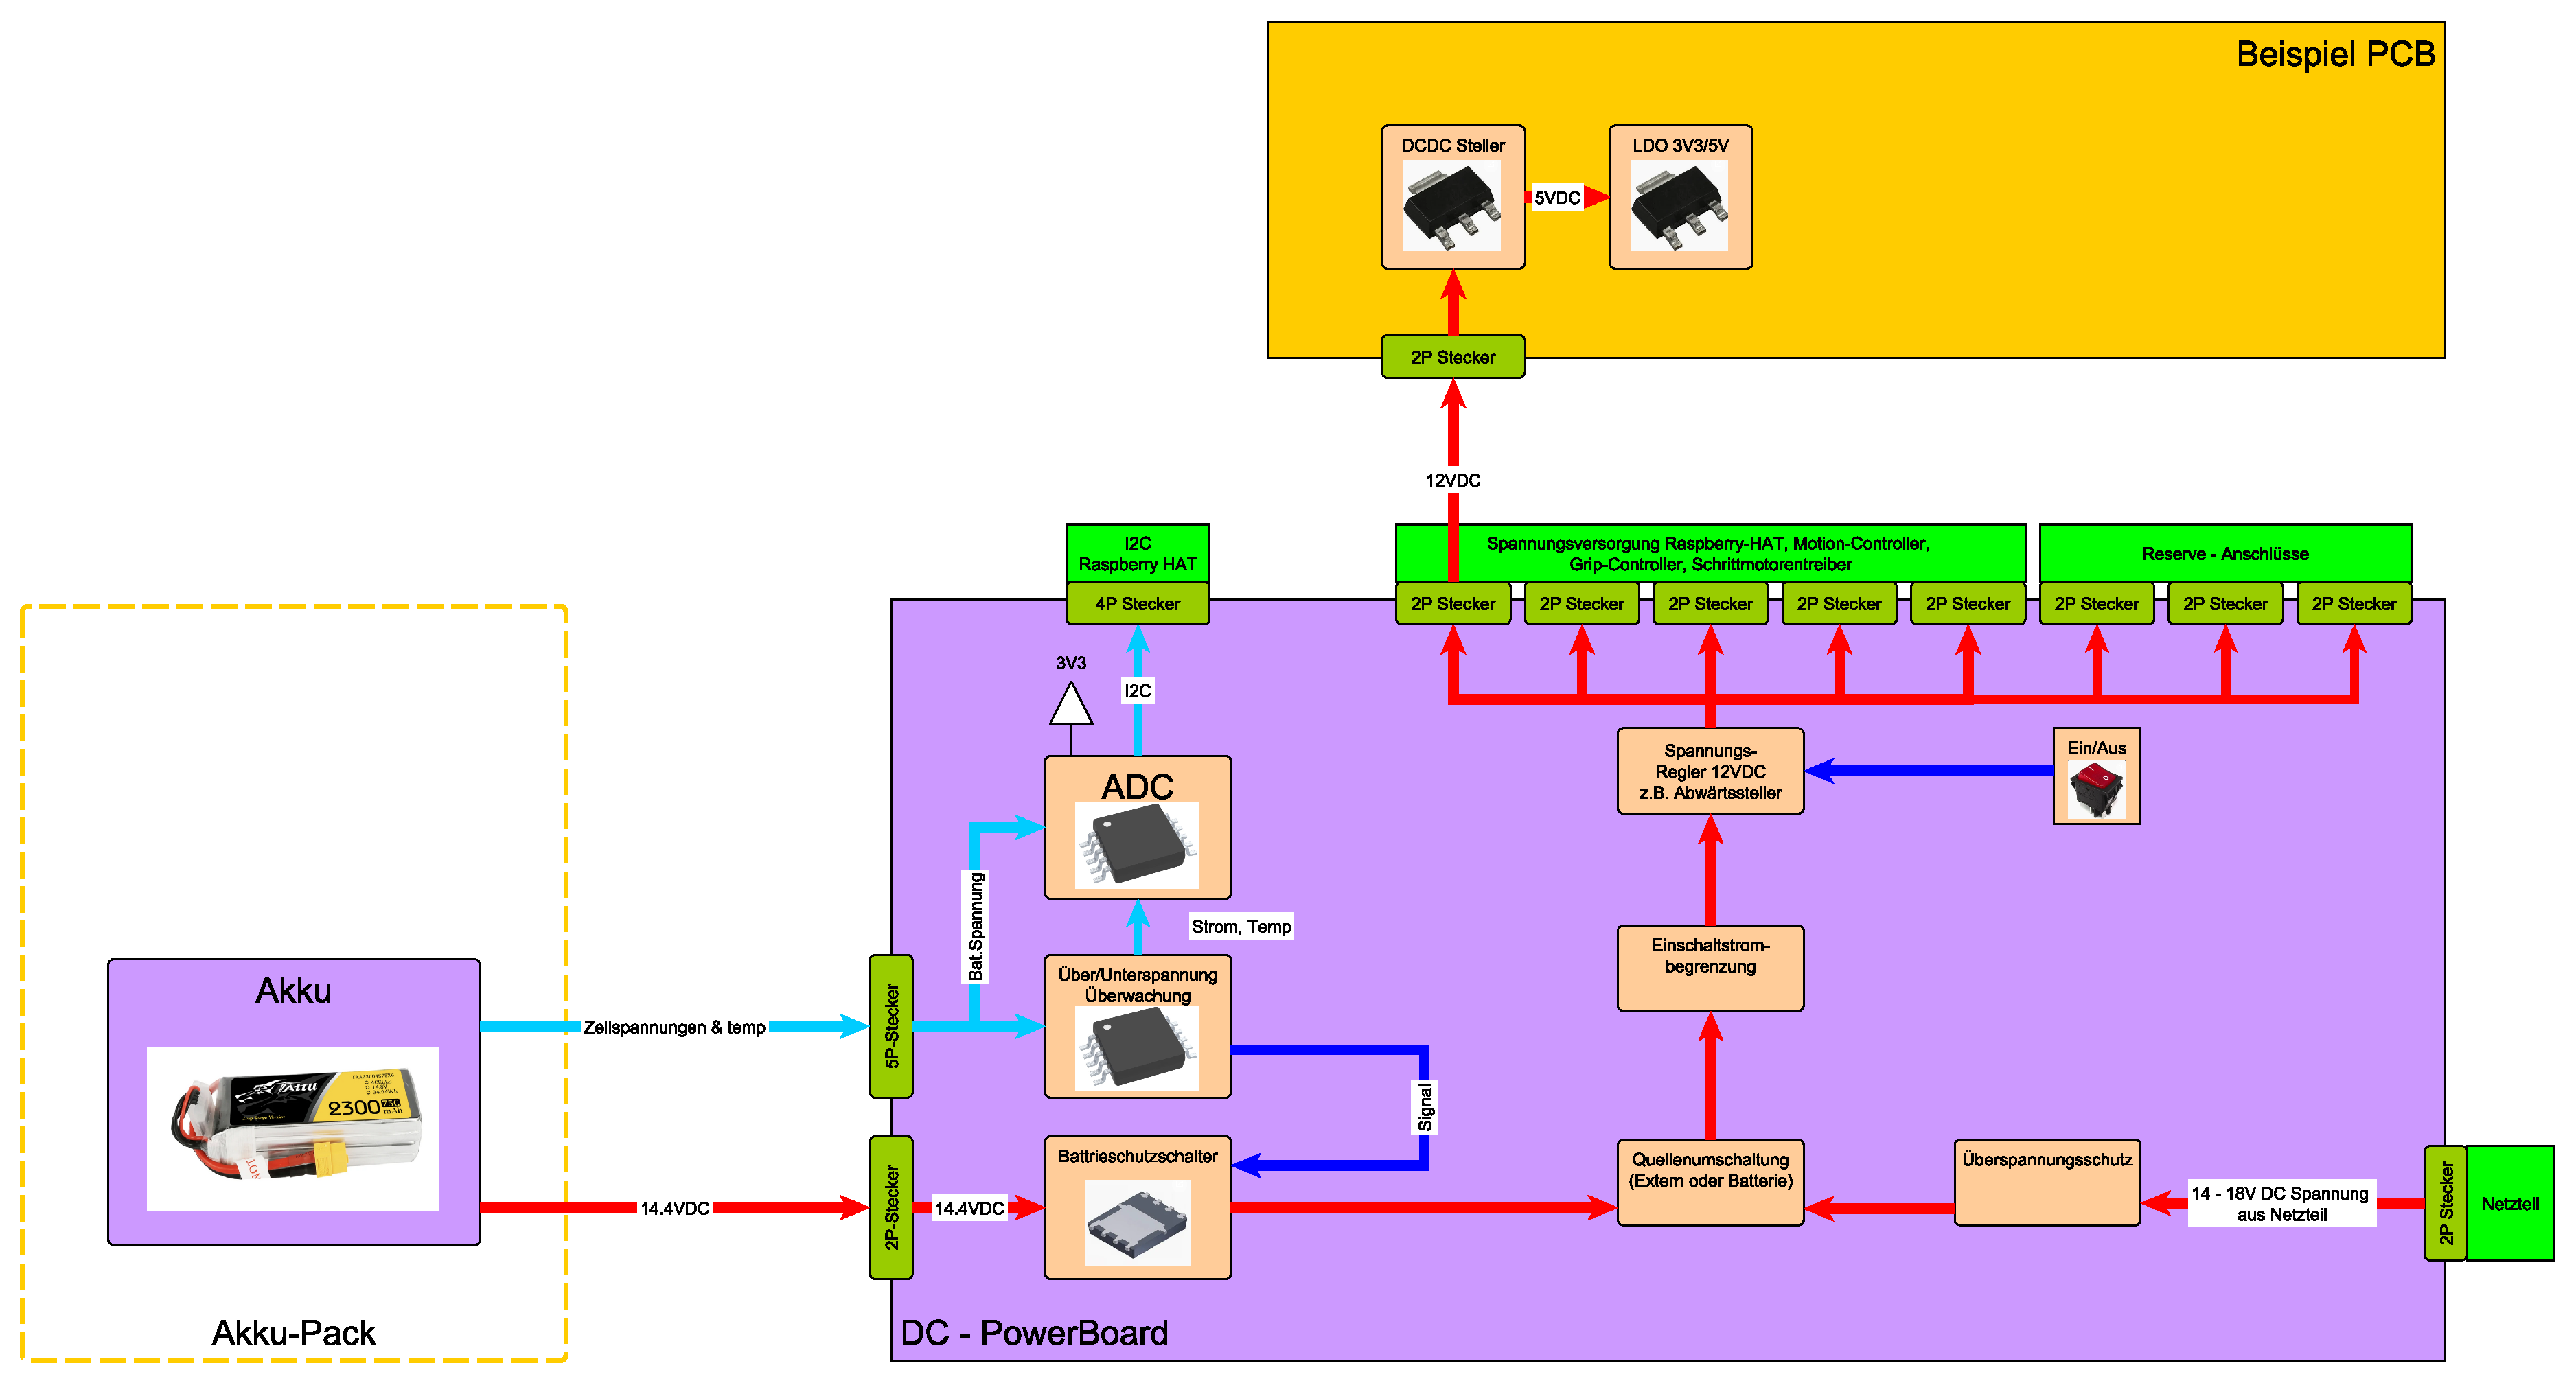
\includegraphics[width = 1\linewidth]{fig_Bordnetz/PowerBoard-Blockschaltbild.pdf}
    \caption{PowerBoard Blockschaltbild}~\label{PowerBoard_Blockschaltbild}
\end{figure}

\paragraph{PowerBoard-PCB}
Die Ausgangsspannung von 14,4V wird auf dem selbstentwickelten PowerBoard mit
einem Abwärtsregler auf 12V geregelt. Dieses Board bietet auch die Möglichkeit,
von einem Netzteil im Bereich von 12 bis 18V versorgt zu werden, wobei die
Batterie automatisch abgeschaltet wird. Damit ist der Roboter bei Entwicklungs-
und Einrichtaufgaben nicht zwingend auf die Energieversorgung über die Batterie
angewiesen, sondern kann auch über ein Netzteil betrieben werden.

Batteriespannung und -strom werden über einen ADC überwacht und können über
$I^2C$ vom Raspberry Pi ausgelesen werden.

Die Batterieschutzschaltung überwacht die Zellspannungen des LiPo-Akkus einzeln
und trennt den Akku vom Roboter, wenn eine der Zellen in den
Unterspannungsbereich gerät. Dieser Zustand wird durch eine rot leuchtende LED
angezeigt. Der Zellenausgleich wird nicht am Roboter selbst durchgeführt. Zu
diesem Zweck wurde ein Ladegerät aus dem Modellbaubereich beschafft, das in der
Lage ist, die Zellen aktiv auszubalancieren.

Der Schaltplan dieser Platine und das Layout sind im Anhang beigefügt.
Abbildung~\ref{PowerBoard_Ansicht} zeigt eine 3D-Ansicht dieser Platine.

\begin{figure}[H]
    \centering
    \includegraphics[width = 0.75\linewidth]{fig_Bordnetz/PowerDistributionBoard.jpg}
    \caption{Ansicht PowerBoard}~\label{PowerBoard_Ansicht}
\end{figure}

\paragraph{GND-Konzept}

Abbildung~\ref{fig:GND_Konzept} zeigt das GND-Konzept des Roboters. Im
Anschluss wird dieses noch ein wenig ausgeführt.
\begin{figure}[H]
    \centering
    \includegraphics[width = 0.75\linewidth]{fig_Bordnetz/Blockschaltbid_GND_Konzept.pdf}
    \caption{Blockschaltbild GND-Konzept}~\label{fig:GND_Konzept}
\end{figure}

Da sich auf dem Roboter mehrere Leiterplatten befinden, die miteinander
kommunizieren und interagieren, muss sichergestellt werden, dass sich diese auf
einem ähnlichen Potential befinden. Einfache Überlegungen führen schnell zu der
zu der Schlussfolgerung, dass jede Leiterplatte mit ihren Befestigungsschrauben
auf GND-Potential mit einem leitfähigen Chassis verbunden wird. Wird so
verfahren, können Signalrückführungen nicht genau vorhergesagt werden und es
können sich GND-Schleifen bilden. In Anbetracht der Tatsache, dass sich Motoren
und damit sich ändernde Magnetfelder auf dem Gerät befinden, müssen genau diese
GND-Schleifen vermieden werden und es kann nicht einfach jede Platine leitend
mit der Grundplatte verschraubt werden. Dem wird dadurch entgegengewirkt, dass
jede Leiterplatte eine 2-polige Spannungsversorgung erhält und nur über diese
eine Leitung mit dem GND-Netz verbunden ist. Die Befestigungslöcher sollten
isoliert mit der Grundplatte verbunden werden, damit sich keine GND-Schleifen
über das Gehäuse bilden können. In diesem Fall laufen alle GND-Verbindungen
sternförmig auf dem PowerBoard zusammen. Leichte Potentialunterschiede werden
dadurch ausgeglichen, dass die Kommunikationssignale über eine
RS422-Schnittstelle übertragen werden und somit resistent gegen
Potentialunterschiede von $\pm 15V$ sind.

Wird anstelle eines organischen Materials ein Metallgehäuse für das Chassis
verwendet, so ist der GND eines freien PowerBoard-Ausgangs mit diesem zu
verbinden. Die Leiterplatten selbst werden mit Kunststoffverschraubungen an das
Gehäuse geschraubt, um die Befestigungslöcher von diesem zu isolieren. Auf
diese Weise laufen alle GND-Potentiale sternförmig an einem Punkt auf dem
Chassis zusammen und das Chassis kann nicht als Antenne fungieren.

\end{document}